\documentclass[10pt,a4paper]{article}
\usepackage{amsmath}
\usepackage{amsfonts}
\usepackage{amssymb}
\usepackage{graphicx}
\usepackage[frenchb]{babel}
\usepackage[utf8x]{inputenc}
\graphicspath{{images/}}
\usepackage{parskip}
\usepackage{fancyhdr}
\usepackage{vmargin}
\usepackage{caption}
\usepackage{subcaption}
\usepackage{hyperref}
\setmarginsrb{3 cm}{2.5 cm}{3 cm}{2.5 cm}{1 cm}{1.5 cm}{1 cm}{1.5 cm}

\title{Travaux pratiques avec Weka}                             % Title
\author{Maxime De Wolf}                               % Author
\date{\today}                                           % Date

\makeatletter
\let\thetitle\@title
\let\theauthor\@author
\let\thedate\@date
\makeatother

\pagestyle{fancy}
\fancyhf{}
\rhead{\theauthor}
\lhead{\thetitle}
\cfoot{\thepage}

\begin{document}
   	
   	%%%%%%%%%%%%%%%%%%%%%%%%%%%%%%%%%%%%%%%%%%%%%%%%%%%%%%%%%%%%%%%%%%%%%%%%%%%%%%%%%%%%%%%%%
   	
   	\begin{titlepage}
   		\centering
   		\vspace*{0.5 cm}
   		
\includegraphics[scale = 0.75]{UMONS}\\[1.0 cm]   % University Logo
   		\textsc{\LARGE Université de Mons}\\[2.0 cm]   % University Name
   		\textsc{\large Datawarehousing and datamining}\\[0.5 cm]               % Course Name
   		\rule{\linewidth}{0.2 mm} \\[0.4 cm]
   		{ \huge \bfseries \thetitle}\\
   		\rule{\linewidth}{0.2 mm} \\[1.5 cm]
   		
   		\begin{minipage}{0.4\textwidth}
   			\begin{flushleft} \large
   				\emph{Auteur:}\\
   				\theauthor
   			\end{flushleft}
   		\end{minipage}~
   		\begin{minipage}{0.4\textwidth}
   			\begin{flushright} \large
                                 % Your Student Number
   			\end{flushright}
   		\end{minipage}\\[2 cm]
   		
   		{\large \thedate}\\[2 cm]
   		
   		\vfill
   		
   	\end{titlepage}
   	
   	%%%%%%%%%%%%%%%%%%%%%%%%%%%%%%%%%%%%%%%%%%%%%%%%%%%%%%%%%%%%%%%%%%%%%%%%%%%%%%%%%%%%%%%%%
   	
   	\tableofcontents
   	\newpage
   	
   	%%%%%%%%%%%%%%%%%%%%%%%%%%%%%%%%%%%%%%%%%%%%%%%%%%%%%%%%%%%%%%%%%%%%%%%%%%%%%%%%%%%%%%%%%
   	
   	\section{Weka: Tutoriel}
   	
	   	\subsection{Questions 17.1.9 et 17.1.10}
		   	Ces questions portent sur l'arbre de décision crée à partir du fichier \textit{iris.arff}. Voici donc l'arbre de décision obtenu:
		   	
		   	\begin{figure}[h]
		   		\begin{center}
		   			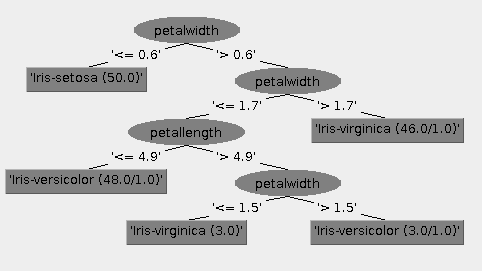
\includegraphics[width=0.3\linewidth]{IrisTree}
		   		\end{center}
		   		\caption{Arbre de décision du \textit{dataset iris.arff}}
		   		\label{fig-Iris-tree}
		   	\end{figure}
		   	
		   	\subsubsection*{Question 17.1.9}
			   	Cette question consiste à évaluer la qualité de cet arbre (Figure \ref{fig-Iris-tree}) grâce à différentes options de tests. Ici, on effectuera ces tests une première fois avec le \textit{dataset} complet et la $2^{e}$ fois avec la technique \textit{10-fold cross-validation}. Nous comparons ensuite les résultats obtenus sur base des 2 \textit{confusion matrix}:\\
	   			
	   			\begin{table}[h]
	   				\centering
					\begin{subtable}{0.4\textwidth}
						\centering
						\caption{\textit{Dataset} complet}
						\begin{tabular}{|c|c|c|l|}
							\hline
							a & b & c & \\ 
							\hline
							50 & 0 & 0 & a = Iris-setosa\\
							\hline
							0 & 49 & 1 & b = Iris-versicolor\\
							\hline
							0 & 2 & 48 & c = Iris-virginica\\
							\hline
						\end{tabular}
					\end{subtable}%
					\begin{subtable}{0.4\textwidth}
						\centering
						\caption{\textit{10-fold cross-validation}}
						\begin{tabular}{|c|c|c|l|}
							\hline
							a & b & c & \\ 
							\hline
							49 & 1 & 0 & a = Iris-setosa\\
							\hline
							0 & 47 & 3 & b = Iris-versicolor\\
							\hline
							0 & 2 & 48 & c = Iris-virginica\\
							\hline
						\end{tabular}
					\end{subtable}
					\caption{\textit{Confusion matrix} obtenues grâce à deux méthodes de test différentes}
	   			\end{table}
 
				 Nous remarquons que le test sur le \textit{dataset} complet classifie correctement $98\%$ des instances tandis que ce chiffre descend à $96\%$ avec le test \textit{10-fold cross-validation}. Tester le modèle avec le \textit{dataset} complet est une mauvaise idée car il donne une estimation optimiste de la qualité du modèle. En revanche, \textit{10-fold cross-validation} permet de se faire une bonne idée de la généralisation du modèle et offre donc une meilleure mesure de qualité.
				 
			\subsubsection*{Question 17.1.10}
			
				En observant la localisation de ces erreurs, nous remarquons que certaines instances de classe \textit{Iris-Verginica} ont des valeurs d'attributs équivalentes à celles d'instance de classe \textit{Iris-Versicolor}. Le modèle n'a donc aucune chance de les différencier si nous voulons éviter l'\textit{overfitting}. D'autre part, nous remarquons que l'instance de classe \textit{Iris-Setosa} qui a été mal identifier aurait dû être correctement classé selon l'arbre de décision final obtenu. 
		
		\subsection{Questions 17.2.4 à 17.2.11}
		
			\subsubsection*{Question 17.2.4}
				Le but de cette question est d'étudier la précision du classificateur \textit{5-nearest neighbor} en fonction des attributs utilisés lors de cette classification. Ici, nous exécutons cette algorithme sur le \textit{dataset glass.arff} et nous le test grâce à la technique \textit{10-fold cross-validation}. Les résultats ainsi obtenus sont résumés dans la table suivante:
				
				\begin{table}[h]
					\centering
					\caption{Précision obtenue en utilisant \textit{IBk} pour différents sous-ensemble d'attributs}
					\begin{tabular}{|c|c|c|}
						\hline
						Nombre d'attributs & Attribut retiré & Précision de la classification\\
						\hline
						9 & $\emptyset$ & 67.757 \\
						\hline
						8 & Si & 71.4953 \\
						\hline
						7 & Fe & 73.3645 \\
						\hline
						6 & Al & 73.3645 \\
						\hline
						5 & & \\
						\hline
						4 & & \\
						\hline
						3 & & \\
						\hline
						2 & & \\
						\hline
						1 & & \\
						\hline
						0 & & \\
						\hline
					\end{tabular}
				\end{table}
			
				
   	
   	\section{CoIL Challenge 2000}
   	
          	
\end{document}